\documentclass[
    12pt,
    oneside, % symmetric pagination
    a4paper,
    %english,
    italian
]{book}

\PassOptionsToPackage{dvipsnames}{xcolor} % colori PDF/A

\usepackage{colorprofiles}
% PDF/A
% validate in https://www.pdf-online.com/osa/validate.aspx
\usepackage[a-1a,mathxmp]{pdfx}[2018/12/22]
%\usepackage{amsmath,amssymb,amsthm} % matematica
\usepackage[T1]{fontenc}
\usepackage[utf8]{inputenc}
\usepackage[italian]{babel}
\usepackage{bookmark}
\usepackage{caption}
\usepackage{chngpage, calc} % centra il frontespizio
\usepackage{csquotes} % gestisce automaticamente i caratteri (")
\usepackage{emptypage} % pagine vuote senza testatina e piede di pagina
\usepackage{epigraph} % per epigrafi
\usepackage{indentfirst} % rientra il primo paragrafo di ogni sezione
\usepackage{graphicx} % immagini
\usepackage[pdfa]{hyperref} % collegamenti ipertestuali
\usepackage{listings} % codici
%\usepackage{microtype} % microtipografia
\usepackage{mparhack,relsize}  % finezze tipografiche
\usepackage{nameref} % visualizza nome dei riferimenti
\usepackage[font=small]{quoting} % citazioni
\usepackage{subfig} % sottofigure, sottotabelle
\usepackage[italian]{varioref} % riferimenti completi della pagina
\usepackage{booktabs} % tabelle
\usepackage{tabularx} % tabelle di larghezza prefissata
\usepackage{longtable} % tabelle su più pagine
\usepackage{ltxtable} % tabelle su più pagine e adattabili in larghezza
\usepackage[toc, acronym, automake]{glossaries}
\usepackage[backend=biber, style=verbose-ibid, hyperref, backref]{biblatex}
\usepackage{lmodern}
\usepackage[top=3cm, bottom=2.75cm, right=3cm, left=3.75cm]{geometry} % 1in+17pt+0.6cm
\usepackage{fancyhdr}
\usepackage{lipsum}
\usepackage{setspace}
\usepackage{titlesec}
% Load variables
\newcommand{\myName}{Paolino Paperino}
\newcommand{\myStudentID}{1234567}
\newcommand{\myTitle}{Lorem ipsum dolor sit amet, consectetur adipisci elit.}
\newcommand{\myUni}{Università degli Studi di Padova}
\newcommand{\myDepartment}{Dipartimento di Matematica ``Tullio Levi-Civita''}
\newcommand{\myFaculty}{Corso di Laurea in Informatica}
\newcommand{\myDegree}{Tesi di Laurea Triennale}
\newcommand{\profTitle}{Prof.}
\newcommand{\myProf}{Cognome Nome}
\newcommand{\myAA}{20XX-20XX}
\newcommand{\myLocation}{Padova}
\newcommand{\myTime}{Mese 20XX}
% Acronyms
\newacronym{api}{API}{Application Program Interface}
\newacronym{sdk}{SDK}{Software Development Kit}
\newacronym{uml}{UML}{Unified Modeling Language}

% Glossary
\newglossaryentry{apig}{
    name={API},
    text={Application Program Interface},
    sort=api,
    description={In computer science, an API is a set of procedures available to programmers, typically grouped to form a toolkit for a specific task within a program. Its purpose is to provide an abstraction, usually between hardware and the programmer or between low-level and high-level software, simplifying the programming process}
}

\newglossaryentry{sdkg}{
    name={SDK},
    text={Software Development Kit},
    sort=sdk,
    description={A Software Development Kit (SDK) is a collection of development tools in one installable package, facilitating application creation by providing a compiler, debugger, and sometimes a software framework. SDKs are typically specific to a hardware platform and operating system combination. Many application developers use specific SDKs to enable advanced functionalities such as advertisements, push notifications, etc}
}

\newglossaryentry{umlg}{
    name={UML},
    text={Unified Modeling Language},
    sort=uml,
    description={In software engineering, Unified Modeling Language (UML) is a modeling and specification language based on the object-oriented paradigm. UML serves as a "lingua franca" in the object-oriented design and programming community. Much of the industry literature uses UML to describe analytical and design solutions in a concise and understandable way for a broad audience}
}

\newglossaryentry{TermineSenzaAcronimo}{
    name={Nome del termine},
    sort=termine senza acronimo,
    description={Descrizione}
}

% Define custom colors
\definecolor{hyperColor}{HTML}{0B3EE3}
\definecolor{tableGray}{HTML}{F5F5F7}

% Set line height
\linespread{1.5}

% Custom hyphenation rules
\hyphenation {
    e-sem-pio
    ex-am-ple
}

% Images path
\graphicspath{{img/}}

% Force page color, as some editors set a grayish color as default
\pagecolor{white}

% Better spacing for footnotes
\setlength{\skip\footins}{5mm}
\setlength{\footnotesep}{5mm}

\setlength{\headheight}{14.5pt}
\addtolength{\topmargin}{-2.45pt}

% Listings setup
\lstset{
    language=[LaTeX]Tex,%C++,
    keywordstyle=\color{RoyalBlue}, %\bfseries,
    basicstyle=\small\ttfamily,
    %identifierstyle=\color{NavyBlue},
    commentstyle=\color{Green}\ttfamily,
    stringstyle=\rmfamily,
    numbers=none, %left,%
    numberstyle=\scriptsize, %\tiny
    stepnumber=5,
    numbersep=8pt,
    showstringspaces=false,
    breaklines=true,
    frameround=ftff,
    frame=single
}

% Add a subscript G to a glossary entry
\newcommand{\glox}{\textsubscript{\textbf{\textit{G }}}}

% If the subscript G is followed by a punctuation character, or anything else, you need to use \gloxspacing to prevent rendering issues, where the characters collide. Example in Chapter 7
\newcommand{\gloxspacing}{\hspace{-0.3em}}

% Improvements the paragraph command
\titleformat{\paragraph}
{\normalfont\normalsize\bfseries}{\theparagraph}{1em}{}
\titlespacing*{\paragraph}
{0pt}{3.25ex plus 1ex minus .2ex}{1.5ex plus .2ex}

% Define use case environment
\newcounter{usecasecounter} % define a counter
\setcounter{usecasecounter}{0} % set the counter to some initial value
% Parameters
% #1: ID
% #2: Nome
\newenvironment{usecase}[2]{
    \renewcommand{\theusecasecounter}{\usecasename #1}  % this is where the display of the counter is overwritten/modified
    \refstepcounter{usecasecounter} % increment counter
    \vspace{2em}
    \par \noindent % start new paragraph
    {\normalsize \textbf{\usecasename #1: #2}} % display the title before the content of the environment is displayed
    \vspace{.5em}
}{
    \medskip
}
\newcommand{\usecasename}{UC}
\newcommand{\usecaseactors}[1]{\textbf{\\Attori Principali:} #1}
\newcommand{\usecasepre}[1]{\textbf{\\Precondizioni:} #1}
\newcommand{\usecasedesc}[1]{\textbf{\\Descrizione:} #1}
\newcommand{\usecasepost}[1]{\textbf{\\Postcondizioni:} #1}
\newcommand{\usecasealt}[1]{\textbf{\\Scenario Alternativo:} #1}

% Define risks environment
\newcounter{riskcounter} % define a counter
\setcounter{riskcounter}{0} % set the counter to some initial value
% Parameters
% #1: Title
\newenvironment{risk}[1]{
    \refstepcounter{riskcounter} % increment counter
    \par \noindent % start new paragraph
    \textbf{\arabic{riskcounter}. #1} % display the title before the content of the environment is displayed
}{
    \par\medskip
}
\newcommand{\riskname}{Rischio}
\newcommand{\riskdescription}[1]{\textbf{\\Descrizione:} #1.}
\newcommand{\risksolution}[1]{\textbf{\\Soluzione:} #1.}

% Apply fancy styling to pages
\pagestyle{fancy}
\fancyhf{}
\fancyhead[L]{\leftmark} % Places Chapter N. Chatper title on the top left
\fancyfoot[C]{\thepage} % Page number in the center of the footer

% Adds a blank page while increasing the page number
\newcommand\blankpage{ 
    \clearpage
    \begingroup
      \null
      \thispagestyle{empty}
      \hypersetup{pageanchor=false}
      \clearpage
    \endgroup
}

% Increase page numbering
\newcommand\increasepagenumbering{
    \addtocounter{page}{+1}
}

% Make glossaries and bibliography
\makeglossaries
\bibliography{appendix/bibliography}
\defbibheading{bibliography} {
    \cleardoublepage
    \phantomsection
    \addcontentsline{toc}{chapter}{\bibname}
    \chapter*{\bibname\markboth{\bibname}{\bibname}}
}
\glsaddall

% Set up hyperlinks
\hypersetup{
    colorlinks=true,
    linktocpage=true,
    pdfstartpage=1,
    pdfstartview=,
    breaklinks=true,
    pdfpagemode=UseNone,
    pageanchor=true,
    pdfpagemode=UseOutlines,
    plainpages=false,
    bookmarksnumbered,
    bookmarksopen=true,
    bookmarksopenlevel=1,
    hypertexnames=true,
    pdfhighlight=/O,
    allcolors = hyperColor
}

% Set up captions
\captionsetup{
    tableposition=top,
    figureposition=bottom,
    font=small,
    format=hang,
    labelfont=bf
}

\date{}

\hypersetup{pdfstartview=}
\begin{document}
    %\layout
    \frontmatter
    \begin{titlepage}
    \begin{center}
        \begin{Large}
            \textbf{\myUni}\\
        \end{Large}

        \vspace{5pt}

        \begin{large}
            \textsc{\myDepartment}\\
        \end{large}

        \vspace{5pt}

        \begin{large}
            \textsc{\myFaculty}\\
        \end{large}

        \vspace{25pt}
        
        \begin{figure}[htbp]
            \centering
            
\includegraphics[alt={Emblema dell'Università degli Studi di Padova}, height=6cm]{img/logo_unipd.jpeg}
        \end{figure}

        
        \begin{Large}
            \textbf{\myTitle}\\
        \end{Large}

        \vspace{5pt}

        \begin{large}
            \textit{\myDegree}\\
        \end{large}

        \vspace{50pt}
        
        \begin{normalsize}
            \begin{flushleft}
                \textit{Relatore}\\
                \vspace{3pt}
                \profTitle\ \myProf
            \end{flushleft}

            \vspace{-48pt}
            
            \begin{flushright}
                \textit{\graduateTitle}\\
                \vspace{3pt}
                \myName\\
                \vspace{3pt}
                Matricola \myStudentID
            \end{flushright}
        \end{normalsize}

        \vspace*{\fill}
        
        \line(1, 0){338} \\
        \begin{normalsize}
            \textsc{Anno Accademico \myAA}
        \end{normalsize}
    \end{center}
\end{titlepage}

    \increasepagenumbering % increase the page numbrering by 1, in order to cout the frontispiece
    \clearpage
\phantomsection
\thispagestyle{empty}
\hfill
\vfill

{\small\noindent\textcopyright\ \myName, \myTime. Tutti i diritti riservati. \myDegree: ``\textit{\myTitle}'', \myUni, \myDepartment.}
    \cleardoublepage
\phantomsection
\pdfbookmark{Ringraziamenti}{Ringraziamenti}

\begin{flushright}{
    \slshape
    ``Colui il quale ha inseguito e sconfitto i demoni Sem, che ora vagano per il mondo, domandandosi: «ma nü, chi sëm?»''} \\
    \medskip
    --- Il grande Pdor, figlio di Kmer, della tribù di Ishtar, della terra desolata dei Kfnir, uno degli ultimi sette saggi: Pfulur, Galér, Astaparigna, Sùsar, Param, Fusus e Tarìm.
\end{flushright}
\bigskip

\begingroup
\let\clearpage\relax
\let\cleardoublepage\relax
\let\cleardoublepage\relax

\chapter*{Ringraziamenti}

\noindent Desidero esprimere la mia gratitudine al professor \myProf, mio relatore, per l'aiuto e il sostegno che mi ha dato durante la stesura dell'elaborato.

\noindent Vorrei anche ringraziare, con affetto, i miei genitori per il loro sostegno, il grande aiuto e la loro presenza in ogni momento durante gli anni di studio.

\noindent Desidero poi ringraziare i miei amici per i bellissimi anni trascorsi insieme e le mille avventure vissute.
\bigskip

\noindent{\myLocation, \myTime}
\hfill \textit{Giovanni} %\myName

\endgroup

    \cleardoublepage
\phantomsection
\pdfbookmark{Compendio}{Compendio}
\begingroup
\let\clearpage\relax
\let\cleardoublepage\relax

\chapter*{Sommario}

Il presente documento descrive il lavoro svolto durante il periodo di stage...

\endgroup
\vfill

    \blankpage % example of a blank page, that also increases the page couter by 1
    \cleardoublepage
\pdfbookmark{\contentsname}{tableofcontents}
\setcounter{secnumdepth}{5}  % Numbering depth for sections
\setcounter{tocdepth}{5}     
% Depth of entries in the table of contents

\tableofcontents
%\markboth{\contentsname}{\contentsname}
\clearpage

\begingroup
    \let\clearpage\relax
    \let\cleardoublepage\relax
    \let\cleardoublepage\relax

    % Figures list
    \phantomsection
    \pdfbookmark{\listfigurename}{lof}
    \listoffigures

    \vspace*{8ex}

    % Tables list
    \phantomsection
    \pdfbookmark{\listtablename}{lot}
    \listoftables

    \vspace*{8ex}
\endgroup

\cleardoublepage
    
    %\cleardoublepage

    \mainmatter
    \chapter{Introduzione}
\label{chap:introduzione}

\begin{figure}[H]
    \centering
    
\includegraphics[alt={Testo alternativo dell'immagine}, width=1\columnwidth]{img/quantum_entanglement.jpeg}
    \caption{Lorem}
    \label{fig:entanglement}
\end{figure}

Introduzione al contesto applicativo.

Lorem Figure \ref{fig:entanglement}

Esempio di utilizzo di un termine nel glossario \gls{api}.

Esempio di citazione in linea \cite{site:agile-manifesto}.

Esempio di citazione nel piè di pagina citazione\footcite{womak:lean-thinking}

\lipsum[1-2]

\section{L'azienda}
\lipsum[1]

\section{L'idea}
Introduzione all'idea dello stage\footcite{article:spooky}.
\lipsum[1-3]

\section{Organizzazione del testo}
\begin{description}
    \item[{\hyperref[chap:processi-metodologie]{Il secondo capitolo}}] descrive ...
    
    \item[{\hyperref[chap:descrizione-stage]{Il terzo capitolo}}] approfondisce ...
    
    \item[{\hyperref[chap:analisi-requisiti]{Il quarto capitolo}}] approfondisce ...
    
    \item[{\hyperref[chap:progettazione-codifica]{Il quinto capitolo}}] approfondisce ...
    
    \item[{\hyperref[chap:verifica-validazione]{Il sesto capitolo}}] approfondisce ...
    
    \item[{\hyperref[chap:conclusioni]{Nel settimo capitolo}}] descrive ...
\end{description}

Riguardo la stesura del testo, relativamente al documento sono state adottate le seguenti convenzioni tipografiche:
\begin{itemize}
	\item gli acronimi, le abbreviazioni e i termini ambigui o di uso non comune menzionati vengono definiti nel glossario, situato alla fine del presente documento;
	\item per la prima occorrenza dei termini riportati nel glossario viene utilizzata la seguente nomenclatura: \gls{apig};
	\item i termini in lingua straniera o facenti parti del gergo tecnico sono evidenziati con il carattere \textit{corsivo}.
\end{itemize}

\begin{listing}[H]
\begin{minted}{c}
#include <stdio.h>
int main() {
    print("Hello, world!");
    return 0;
}
\end{minted}
\caption{Example of code}
\label{listing:a}
\end{listing}

\newpage
    \chapter{Processi e metodologie}
\label{cap:processi-metodologie}

Lorem ipsum dolor sit amet, consectetuer adipiscing elit. Aenean commodo ligula eget dolor. Aenean massa. Cum sociis natoque penatibus et magnis dis parturient montes, nascetur ridiculus mus. Donec quam felis, ultricies nec, pellentesque eu, pretium quis, sem.

\begin{figure}[h]
    \centering
    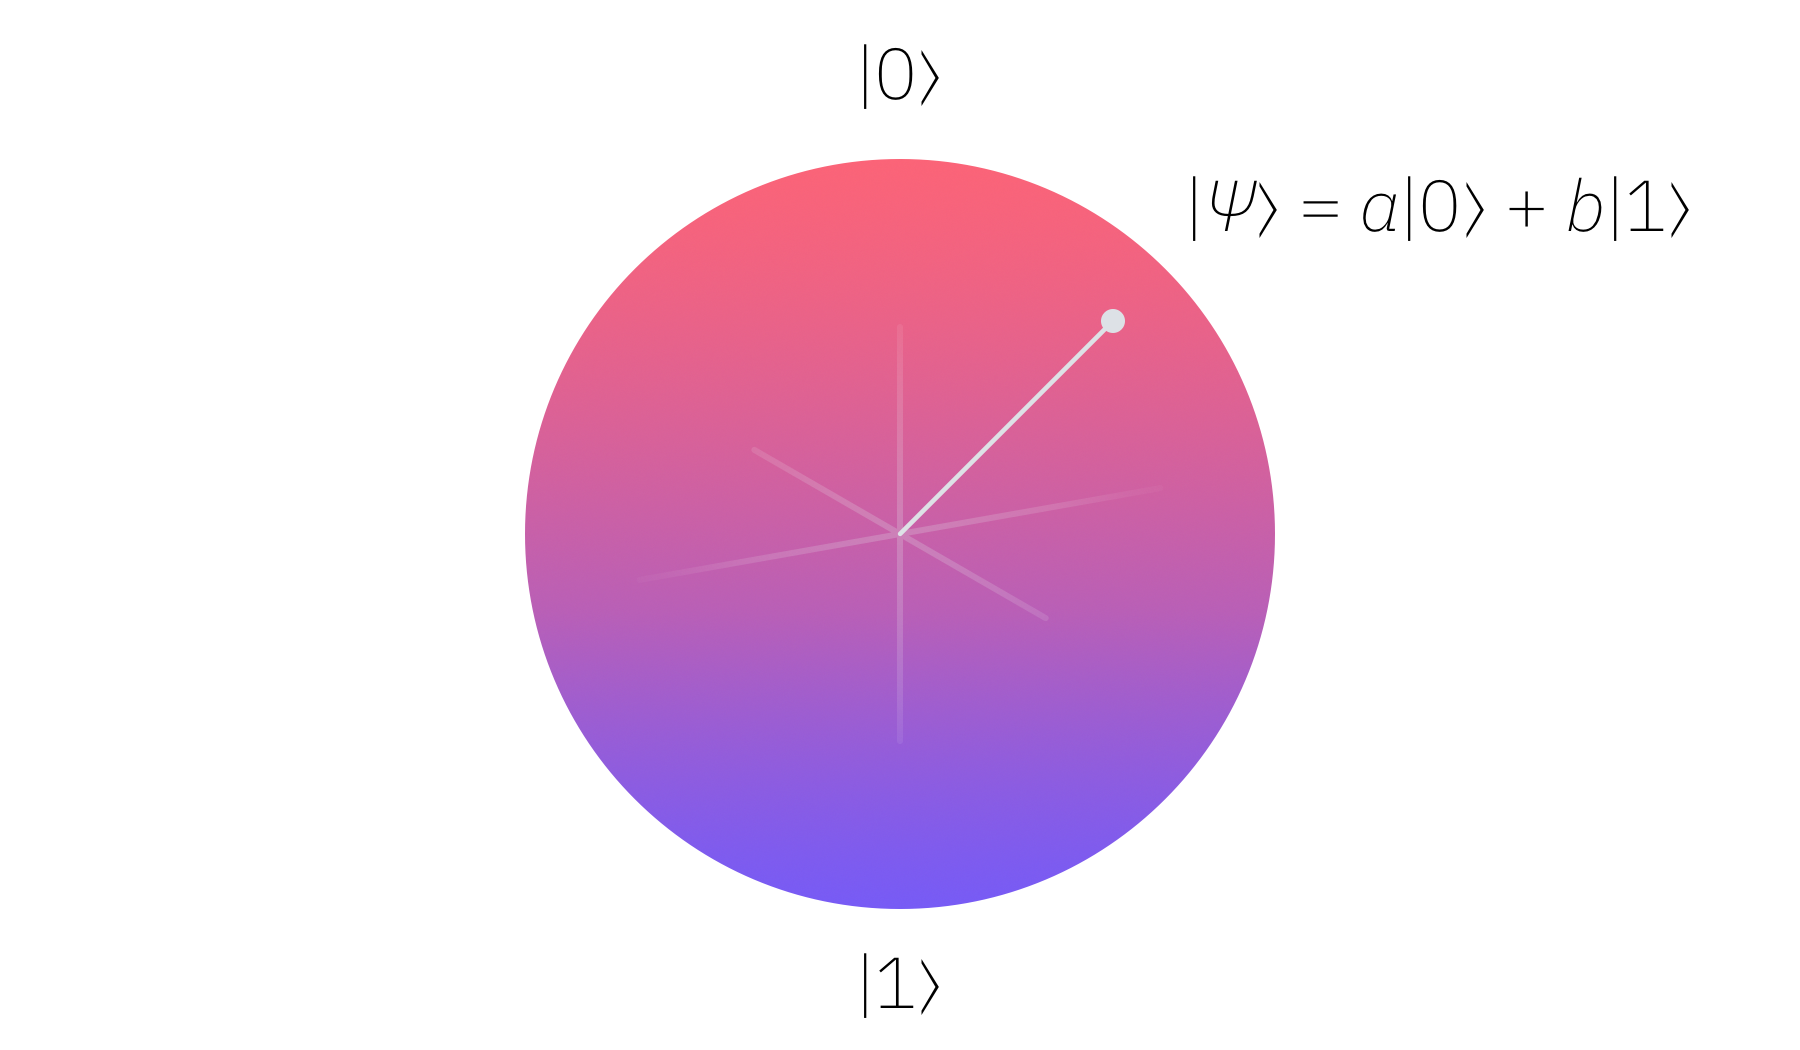
\includegraphics[height=5cm]{img/qubit.png}
    \caption{Lorem}
    \label{fig:qubit}
\end{figure}

\lipsum[1]

\section{Processo sviluppo prodotto}

    \chapter{Descrizione dello stage}
\label{cap:descrizione-stage}

%\intro{Breve introduzione al capitolo}\\

\section{Introduzione al progetto}

\begin{figure}[!ht] 
    \centering 
    
\includegraphics[width=0.5\columnwidth]{pk_estate.jpg} 
    \caption{Caption}
\end{figure}
\lipsum[1]

\section{Analisi preventiva dei rischi}

Durante la fase di analisi iniziale sono stati individuati alcuni possibili rischi a cui si potrà andare incontro.
Si è quindi proceduto a elaborare delle possibili soluzioni per far fronte a tali rischi.

\begin{risk}{Performance del simulatore hardware}
    \riskdescription{le performance del simulatore hardware e la comunicazione con questo potrebbero risultare lenti o non abbastanza buoni da causare il fallimento dei test}
    \risksolution{coinvolgimento del responsabile a capo del progetto relativo il simulatore hardware}
    \label{risk:hardware-simulator} 
\end{risk}

\section{Requisiti e obiettivi}

\section{Pianificazione}
Lorem

\subsection{Ipsum}
Dolor

\subsubsection{Sit}
Amet

\paragraph{Memento}
mori
    \chapter{Analisi dei requisiti}
\label{chap:analisi-requisiti}

\section{Casi d'uso}
Per lo studio dei casi di utilizzo del prodotto sono stati creati dei diagrammi.
I diagrammi dei casi d'uso (in inglese \textit{Use Case Diagram}) sono diagrammi di tipo \gls{uml} dedicati alla descrizione delle funzioni o servizi offerti da un sistema, così come sono percepiti e utilizzati dagli attori che interagiscono col sistema stesso.
Essendo il progetto finalizzato alla creazione di un tool per l'automazione di un processo, le interazioni da parte dell'utilizzatore devono essere ovviamente ridotte allo stretto necessario. Per questo motivo i diagrammi d'uso risultano semplici e in numero ridotto.

\begin{figure}[ht]
    \vspace{2em}
    \centering
    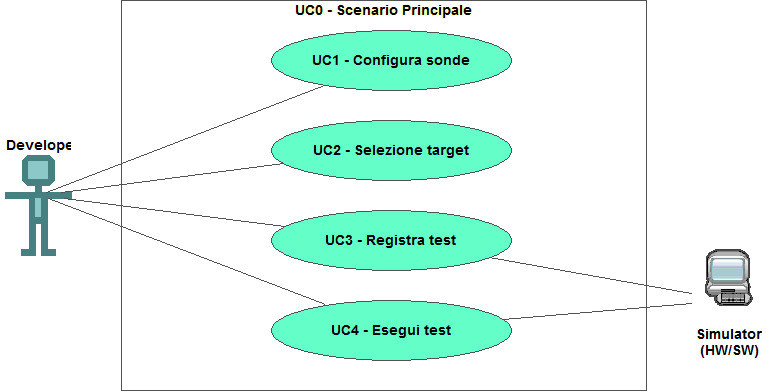
\includegraphics[width=0.75\columnwidth]{img/usecase/scenario-principale.jpeg} 
    \caption{Use Case 0: Scenario principale}
    \label{fig:scenario_principale}
\end{figure}

\begin{usecase}{0}{Scenario principale}
    \usecaseactors{Sviluppatore applicativi.}
    \usecasepre{Lo sviluppatore è entrato nel plugin di simulazione all'interno dell'IDE.}
    \usecasedesc{La finestra di simulazione mette a disposizione i comandi per configurare, registrare o eseguire un test.}
    \usecasepost{Il sistema è pronto per permettere una nuova interazione.}
    \label{uc:uc_scenario_principale}
\end{usecase}

\begin{usecase}{1}{Gestione Utente}
    \usecaseactors{Amministratore, Utente Registrato.}
    \usecasepre{L'utente deve essere autenticato nel sistema.}
    \usecasedesc{L'utente può gestire le informazioni del proprio profilo.}
    \usecasepost{Le modifiche vengono salvate nel sistema.}
    \usecasealt{Se l'utente non è autenticato, visualizza un messaggio di errore.}
    \label{uc:uc_casi_uso}
\end{usecase}

\begin{usecase}{2}{Creazione Prodotto}
    \usecaseactors{Amministratore.}
    \usecasepre{L'amministratore ha effettuato l'accesso al sistema.}
    \usecasedesc{L'amministratore può aggiungere un nuovo prodotto al catalogo.}
    \usecasepost{Il nuovo prodotto viene aggiunto con successo.}
    \usecasealt{Se i campi obbligatori non sono compilati, visualizza un messaggio di errore.}
    \label{uc:uc_creazione_prodotto}
\end{usecase}

\section{Tracciamento dei requisiti}
Da un'attenta analisi dei requisiti e degli use case effettuata sul progetto è stata stilata la tabella che traccia i requisiti in rapporto agli use case.\\
Sono stati individuati diversi tipi di requisiti e si è quindi fatto utilizzo di un codice identificativo per distinguerli.\\
Il codice dei requisiti, dove ogni requisito è identificato con il carattere \textbf{R}, è così strutturato:
\begin{enumerate}
    \item[\textbf{F}:] Funzionale.
    \item[\textbf{Q}:] Qualitativo.
    \item[\textbf{V}:] Di vincolo.
    \item[\textbf{N}:] Obbligatorio (necessario).
    \item[\textbf{D}:] Desiderabile.
    \item[\textbf{Z}:] Opzionale.
\end{enumerate}

Nelle tabelle \ref{tab:requisiti_funzionali}, \ref{tab:requisiti_qualitativi} e \ref{tab:requisiti_vincolo} sono riassunti i requisiti e il loro tracciamento con gli use case delineati in fase di analisi.

\section{Tabelle dei requisiti}
\begin{center}
    \begin{longtable}{|p{2.25cm}|p{7.75cm}|p{2.25cm}|}
    \hline \multicolumn{1}{|c|}{\textbf{Requisito}} & \multicolumn{1}{c|}{\textbf{Descrizione}} & \multicolumn{1}{c|}{\textbf{Use Case}} \\ \hline 
    \endfirsthead
    
    \multicolumn{3}{c}%
    {{\bfseries \tablename\ \thetable{} -- Continuo della tabella}} \\
    \hline \multicolumn{1}{|c|}{\textbf{Requisito}} & \multicolumn{1}{c|}{\textbf{Descrizione}} & \multicolumn{1}{c|}{\textbf{Use Case}} \\ \hline 
    \endhead
    
    \hline \multicolumn{3}{|r|}{{Continua nella prossima pagina...}} \\ \hline
    \endfoot
    \endlastfoot
    
    RFN-1 & L'interfaccia permette di configurare il tipo di sonde del test & UC1 \\
    \hline
    
    \caption{Tabella del tracciamento dei requisiti funzionali.}
    \label{tab:requisiti_funzionali}
    \end{longtable}
\end{center}

\begin{center}
    \begin{longtable}{|p{2.25cm}|p{7.75cm}|p{2.25cm}|}
    \hline \multicolumn{1}{|c|}{\textbf{Requisito}} & \multicolumn{1}{c|}{\textbf{Descrizione}} & \multicolumn{1}{c|}{\textbf{Use Case}} \\ \hline 
    \endfirsthead
    
    \multicolumn{3}{c}%
    {{\bfseries \tablename\ \thetable{} -- Continuo della tabella}} \\
    \hline \multicolumn{1}{|c|}{\textbf{Requisito}} & \multicolumn{1}{c|}{\textbf{Descrizione}} & \multicolumn{1}{c|}{\textbf{Use Case}} \\ \hline 
    \endhead
    
    \hline \multicolumn{3}{|r|}{{Continua nella prossima pagina...}} \\ \hline
    \endfoot
    \endlastfoot
    
    RQD-1n & Le prestazioni del simulatore hardware deve garantire la giusta esecuzione dei test e non la generazione di falsi negativi & - \\
    \hline
    \caption{Tabella del tracciamento dei requisiti qualitativi.}
    \label{tab:requisiti_qualitativi}
    \end{longtable}
\end{center}

\begin{center}
    \begin{longtable}{|p{2.25cm}|p{7.75cm}|p{2.25cm}|}
    \hline \multicolumn{1}{|c|}{\textbf{Requisito}} & \multicolumn{1}{c|}{\textbf{Descrizione}} & \multicolumn{1}{c|}{\textbf{Use Case}} \\ \hline 
    \endfirsthead
    
    \multicolumn{3}{c}%
    {{\bfseries \tablename\ \thetable{} -- Continuo della tabella}} \\
    \hline \multicolumn{1}{|c|}{\textbf{Requisito}} & \multicolumn{1}{c|}{\textbf{Descrizione}} & \multicolumn{1}{c|}{\textbf{Use Case}} \\ \hline 
    \endhead
    
    \hline \multicolumn{3}{|r|}{{Continua nella prossima pagina}} \\ \hline
    \endfoot
    \endlastfoot
    
    RVO-1 & La libreria per l'esecuzione dei test automatici deve essere riutilizzabile & - \\
    \hline
    \caption{Tabella del tracciamento dei requisiti di vincolo.}
    \label{tab:requisiti_vincolo}
    \end{longtable}
\end{center}

\newpage
    \chapter{Progettazione e codifica}
\label{chap:progettazione-codifica}
Breve introduzione al capitolo

\section{Tecnologie e strumenti}
\label{sec:tecnologie-strumenti}
Di seguito viene data una panoramica delle tecnologie e strumenti utilizzati.

\subsection*{Tecnologia 1}
Descrizione Tecnologia 1.

\subsection*{Tecnologia 2}
Descrizione Tecnologia 2

\section{Ciclo di vita del software}
\label{sec:ciclo-vita-software}

\section{Progettazione}
\label{sec:progettazione}

\subsection{Namespace 1}
Descrizione namespace 1.

\section{Design Pattern utilizzati}

\section{Codifica}
Blocco di codice in C
\begin{listing}[H]
\begin{minted}{c}
#include <stdio.h>
int main() {
    print("Hello, world!");
    return 0;
}
\end{minted}
\caption{Example of code}
\label{listing:c}
\end{listing}

\newpage
    \chapter{Verifica e validazione}
\label{chap:verifica-validazione}

\begin{figure}[h!]
    \centering
    
\includegraphics[alt={Testo alternativo dell'immagine}, width=1\columnwidth]{img/quantum_superposition.jpeg}
    \caption{Lorem}
    \label{fig:enter-label}
\end{figure}

\lipsum[1-2]

\newpage
    \chapter{Conclusioni}
\label{chap:conclusioni}

\section{Consuntivo finale}
Ipsum

\section{Raggiungimento degli obiettivi}
Sit amet

\section{Conoscenze acquisite}
% per avere termine di glossario con apice "g" che appare
%Lorem \glsfirstoccur{\gls{sdkg}}
Lorem Ipsum dolor Lorem \gls{sdkg}
% per avere termine di glossario normale
Lorem \gls{apig}

\section{Valutazione personale}
% per avere termine di glossario normale
Lorem \gls{umlg}

\section{Valutazione personale}
Lorem Ipsum dolor Lorem \gls{sdk}

\newpage

    %\appendix
    \pagenumbering{roman}
    \backmatter
    \chapter{Bibliografia}
\label{cap:bibliography}
%\cleardoublepage

\nocite{*}

% Books bibliography
\printbibliography[heading=subbibliography, title={Books}, type=book]

% Articles bibliography
\printbibliography[heading=subbibliography, title={Articles}, type=article]

% Websites bibliography
\printbibliography[heading=subbibliography, title={Websites}, type=online]

    \chapter{Sitografia}
\label{cap:webliography}
\nocite{*}

% Websites bibliography
\printbibliography[heading=subbibliography, title={\null}, type=online]

    \printglossary[type=\acronymtype, title=Acronimi e abbreviazioni, toctitle=Acronimi e abbreviazioni]
    \printglossary[type=main, title=Glossario, toctitle=Glossario]
\end{document}